\chapter{Pomiarowa weryfikacja tezy}

Ostatni etap weryfikacji postawionej w pracy tezy stanowi analiza właściwości metrologicznych przykładowego toru pomiarowego, który stworzony został na potrzeby pracy. Analizowany tor pomiarowy przetwarza zmienny w czasie sygnał napięciowy $s(t)$ o chwilowej wartości napięcia z przedziału $\hat{s}(t) \in~<0;1>~\unit{V}$. W celu dopasowania poziomu sygnału napięcia wejściowego do zakresu napięcia wejściowego przetwornika analogowo-cyfrowego oraz zwiększenia impedancji wejściowej toru pomiarowego, sygnał $s(t)$ podawany jest na wejście wzmacniacza pomiarowego. Sygnał wyjściowy $y(t)$ wzmacniacza przetwarzany jest na postać cyfrową $c(i)$, a następnie po wykonaniu odtwarzania statycznego, podawany jest w postaci wielkości $x(i)$ na wejście jednostki \enquote{DSP}, która dla każdego $j$-tego okna pomiarowego pobiera $N$ próbek tego sygnału i wyznacza na ich podstawie $M$ wartości wielkości wyjściowych wektora $\mathbf{X}(j)$, stosując w tym celu algorytm dyskretnej transformacji falkowej. Schemat blokowy omawianego toru pomiarowego przedstawiono na rysunku~\ref{fig:chain_real}.

\begin{figure}[htb!]
\begin{center}
\includegraphics{obrazki/schemat_real}
\makecaption{fig:chain_real}{Schemat blokowy stworzonego na potrzeby pracy toru pomiarowego będącego obiektem przeprowadzanego eksperymentu}
\end{center}
\end{figure}

Do realizacji układu wzmacniacza pomiarowego zastosowany został wzmacniacz operacyjny \enquote{MCP6002}~\cite{microchip_manual} w konfiguracji nieodwracającej, o docelowym wzmocnieniu wynoszącym~\qty{3.3}{V \per V}. Napięcie zasilania wzmacniacza wynosi~\qty{3.3}{V} i pochodzi ze stabilizatora \enquote{LD1117}~\cite{stm_manual} typu \enquote{LDO} (ang. \enquote{Low Dropout}). Zaproponowana konfiguracja, zgodnie z wcześniejszymi założeniami, zapewnia wysoką impedancję wejściową toru pomiarowego oraz bardzo niską impedancję wyjściową wzmacniacza. Parametry statyczne oraz dynamiczne analizowanego obiektu wymagają identyfikacji, ze względu na niedostateczne informacje zawarte w dokumentacji wykorzystanego układu oraz nieznajomości dokładnego modelu dla zastosowanej aplikacji. Należy zauważyć, że dokładna analiza zastosowanego układu byłaby skomplikowana i nie jest konieczna do oceny jego właściwości metrologicznych związanych z zastosowanie proponowanego w pracy modelu błędu.

Zastosowany przetwornik analogowo-cyfrowy stanowi $12$-bitowy przetwornik wagowy~\enquote{SAR} (ang. \enquote{Successive Approximation Register}), wbudowany w mikrokontroler \enquote{STM32F411}~\cite{stm_f411}. Źródło napięcia odniesienia stanowi w jego przypadku stabilizator \enquote{AP7343}~\cite{diodes_manual} typu \enquote{LDO}, o znamionowym napięciu wyjściowym równym~\qty{3.3}{V}, przyłączony z użyciem dodatkowego filtru LC. Przetwornik analogowo-cyfrowy taktowany jest sygnałem zegarowym o częstotliwości~\qty{24}{MHz}, przy czym próbkowanie wyzwalane jest sygnałem z licznika, którego częstotliwość wyzwalania wynosi $f_{s} = \qty{48}{kHz}$. Na pojedynczy proces konwersji analogowo-cyfrowej przypada kluczowanie napięcia wejściowego, trwające $15$ taktów zegara, po którym następuje konwersja, trwająca $15$ taktów zegara, co w analizowanym przypadku stanowi czas~\qty{625}{ns} dla każdej z operacji. Łączny czas konwersji analogowo-cyfrowej pojedynczej próbki sygnału wejściowego $y(t)$ na jego dyskretną reprezentację $c(i)$ wynosi zatem~\qty{1250}{ns}. Ze względu na typową aplikacje omawianego przetwornika, jego najistotniejsze parametry metrologiczne mogą zostać pozyskane z dokumentacji producenta układu~\cite{stm_f411}. Algorytm odtwarzania statycznego przekształca sygnał $c(i)$ na sygnał $x(i)$ tak, aby stanowił on dyskretną reprezentację sygnału $s(t)$ o czułości \qty{1}{V \per V} względem tego sygnału.

Pozyskane próbki napięcia $x(i)$, stanowiące dyskretną reprezentację sygnału wejściowego $s(t)$, zapisywane są w wektorze $\mathbf{x}(j)$ o długości $N = 128$. Wektor wielkości wejściowych $\mathbf{x}(j)$ podawany jest na wejście algorytmu dyskretnej transformacji falkowej, którego implementacja zrealizowana została z wykorzystaniem instrukcji \enquote{DSP} dostępnych dla zastosowanego mikrokontrolera~\cite{reay_dsp}. Analizowany algorytm wykorzystuje falkę \enquote{spline4:4}~\cite{wang_splinebasics} dla pięciu iteracji procesu dekompozycji sygnału. Zgodnie z równaniem~\eqref{eq:alg_out_mat} wyznaczanych jest $M = 128$ próbek wektora wielkości wyjściowych $\mathbf{X}(j)$, które stanowią wyjście dla pojedynczej $j$-tej serii pomiarowej analizowanego toru pomiarowego. Wartości elementów macierzy transformacji $\mathbf{A}$ zidentyfikowano zgodnie z metodą przedstawioną w równaniu~\eqref{eq:wt_ident}, wykorzystując w tym celu implementacje algorytmu transformacji falkowej dostępną w programie \enquote{GNU Octave}~\cite{pruuvsa_dwt}. Czas obliczeń wynosi w analizowanym przypadku~\qty{1508}{\micro s}, przy czym łączny czas akwizycji pojedynczego wektora próbek wielkości wejściowych wynosi~\qty{2666.6(6)}{\micro s}. Podczas obliczeń stosowane są liczby zmiennoprzecinkowe pojedynczej precyzji o długości słowa $32$-bitów, implementowane sprzętowo przez jednostkę \enquote{FPU} (ang. \enquote{Floating Point Unit}~\cite{cortex_fpu, gcc_manual}.

Przedstawiony tor pomiarowy pracuje w trybie ciągłym, tj. w pojedynczym $j$-tym oknie pomiarowym, podczas pobierania próbek wielkości wejściowych wektora $\mathbf{x}(j)$, wyznaczana jest realizacja wektora wielkości wyjściowych $\mathbf{X}(j-1)$ dla poprzedniej realizacji wektora wielkości wejściowych $\mathbf{x}(j-1)$. Wykorzystywany jest w tym celu kontroler \enquote{DMA} (ang. \enquote{Direct Memory Access}), nadzorujący proces buforowania kolejnych realizacji sygnału $x(i)$, w czasie gdy program główny wykonuje obliczenia dane równaniem~\eqref{eq:alg_out_mat}. Analiza wartości wielkości wyjściowych omawianego toru pomiarowego jest możliwa między innymi po podłączeniu go do komputera klasy \enquote{PC} za pośrednictwem portu \enquote{USB}, przy czym wykorzystywany jest w tym celu układ peryferyjny \enquote{USB OTG Full-Speed}, zintegrowany w zastosowanym mikrokontrolerze. Alternatywną możliwość komunikacji z urządzeniem stanowi interfejs \enquote{UART} (ang. \enquote{Universal Asynchronous Receiver-Transmitter}), natomiast ze względu na ograniczenie szybkości transferu danych przez ten interfejs, nie umożliwia on ciągłego śledzenia wyników pomiarów.

W dalszej części rozdziału opisano najważniejsze źródła błędów analizowanego toru pomiarowego, a następnie wykorzystano zaproponowany w pracy model błędu do opisu właściwości wykazanych sygnałów błędów. Ze względu na fakt, że nie jest znany dokładny model analizowanego toru pomiarowego, przeprowadzono identyfikację jego właściwości, istotnych ze względu na zaproponowany model błędu. W ostatniej części rozdziału opisano przeprowadzony eksperyment pomiarowy, wykorzystujący metodę Monte-Carlo, mający na celu ocenę poprawności przedstawionych rozważań i weryfikacje możliwości praktycznej aplikacji zawartych w pracy propozycji. Poza analizą właściwości metrologicznych zbudowanego toru pomiarowego, przeprowadzona analiza obejmowała również wpływ sygnałów błędów zawartych w przetwarzanej wielkości $s(t)$ na budżet niepewności analizowanego urządzenia. Podczas eksperymentów wykorzystano generator przebiegów arbitralnych, którego rzeczywiste parametry sygnału wejściowego w zależności od wariantu eksperymentu weryfikowano, lub pozostawiano nieznane. Celem omawianego zabiegu było przedstawienie przykładu, w jaki sposób stosując zaproponowany w pracy model błędu należy rozpatrywać omawiane rozbieżności w nastawie parametrów syntezowanego sygnału. Temperatura otoczenia podczas przeprowadzania eksperymentów była stała i wynosiła~\qty{21}{\degreeCelsius}.

\section{Model błędu wielkości wejściowej}

Jako, że w analizowanym przypadku źródło napięciowego sygnału wejściowego $s(t)$ toru pomiarowego stanowi generator przebiegów arbitralnych RIGOL DG1011~\cite{rigol_fawg}, należy uwzględnić jego parametry w budżecie niepewności. Zgodnie z dokumentacją, błąd graniczny nastawy wartości amplitudy $E$ sygnału wyjściowego generatora wynosi:
\begin{equation}
\delta_{E,gr} = \pm \emb{\frac{0.5}{100} \left| E \right| + \frac{0.5}{1000}} ~\unit{V} \label{eq:pom_gen_amperr_max},
\end{equation}
natomiast błąd graniczny nastawy składowej stałej $D$ sygnału wyjściowego wynosi:
\begin{equation}
\delta_{D,gr} = \pm \emb{\frac{0.5}{100} \left| D \right| + \frac{2}{1000}} ~\unit{V} \label{eq:pom_gen_shferr_max},
\end{equation}
przy czym omawiane wielkości $E$ oraz $D$ wyrażone są w woltach. Na podstawie powyższych zależności należy oszacować przedział dla zadanego poziomu ufności, w jakim znajduje się $\alpha$ wartości realizacji błędu nastawy amplitudy oraz błędu nastawy składowej stałej. Zgodnie z wytycznymi zawartymi w~\cite{jcgm_guide} i przyjętym w pracy poziomem ufności $\alpha = 95\%$ zapisać można:
\begin{gather}
U_{E} \emb{x} = c_{u} \cdot \sigma_{E} \emb{x} = c_{u} \frac{\left| \delta_{E,gr} \emb{x} \right|}{\sqrt{3}} = 1.65 \frac{\num{5e-3} \left| x \right| + \num{0.5e-3}}{\sqrt{3}} ~\unit{V} \label{eq:pom_gen_amperr_unc}, \\
U_{D} \emb{x} = c_{u} \cdot \sigma_{D} \emb{x} = c_{u} \frac{\left| \delta_{D,gr} \emb{x} \right|}{\sqrt{3}} = 1.65 \frac{\num{5e-3} \left| x \right| + \num{2e-3}}{\sqrt{3}} ~\unit{V} \label{eq:pom_gen_shferr_unc}.
\end{gather}
gdzie $x$ jest wartością zadaną dla analizowanego parametru wyrażoną w woltach. Należy zauważyć, że w przypadku pojedynczego przyrządu, omawiane rozbieżności w nastawie przedstawionych parametrów stanowią systematyczne źródło błędów, a ich wpływ nożna skorygować przeprowadzając kalibrację przyrządu. Niezależnie od wykonania kalibracji przyrządu, dla syntezowanego sygnału sinusoidalnie zmiennego o wartości zadanej amplitudy $\dot{E}_{s,o}$ oraz składowej stałej o wartości zadanej $\dot{D}_{s,o}$, sygnał $s(t)$ na wyjściu przyrządu opisać można w dziedzinie czasu za pomocą równań:
\begin{gather}
\dot{s} \emb{t} = \dot{E}_{s,o} \sin \emb{\omega_{s,o} t} \label{eq:pom_gen_out_ideal}, \\
\tilde{s} \emb{t} = \dot{s} \emb{t} + e_{s,s} \emb{t} + e_{s,d} \emb{t} + e_{s,r} \emb{t}\label{eq:pom_gen_out_real},
\end{gather}
gdzie symbolem $e_{s,s}(t)$ oznaczono błąd statyczny, symbolem $e_{s,s}(t)$ błąd dynamiczny, natomiast symbolem $e_{s,r}(t)$ oznaczono sygnał błędu losowego. Deterministyczna postać sygnałów błędów $e_{s,s}(t)$ oraz $e_{s,d}(t)$ nie jest znana, jeżeli dla konkretnego modelu urządzenia nie zostanie wykonana kalibracja. Jeżeli eksperyment nie zakłada wykonywania kalibracji stosowanego przyrządu, koniczne jest wskazanie opisu przedstawionych sygnałów w kategorii probabilistycznej, przy czym należy wskazać parametry tych sygnałów, których wartość umożliwi wskazanie niepewności rozszerzonej związanej z ich wpływem o zadanym poziomie ufności $\alpha$. Po wykonaniu kalibracji oraz wykonaniu korekty błędów systematycznych można przyjąć, że $e_{s,s}(t) = 0$ oraz $e_{s,d}(t) = 0$. W przypadku, gdy błędy systematyczne nie zostaną skorygowane po wykonaniu kalibracji, należy opisać deterministycznie przebiegi sygnałów związanych z tymi błędami oraz wskazać wartości ich wariancji i niepewności rozszerzonej.

W przypadku sygnału błędu statycznego $e_{s,s}(t)$ przyjąć można, że błąd ten powodowany jest rozbieżnością nastawy wartości składowej stałej. Wartość realizacji tego sygnału jest stała dla zadanej wartości parametru $\dot{D}_{s,o}$, natomiast jego parametry określać może wariancja oraz niepewność rozszerzona, definiowane na podstawie równania~\eqref{eq:pom_gen_amperr_unc}. Zatem, w przypadku braku kalibracji przyrządu zapisać można:
\begin{gather}
e_{s,s} \emb{t} = E_{s,e,0} \emb{\dot{D}_{s,o}} = \tilde{D}_{s,o} - \dot{D}_{s,o} \label{eq:pom_gen_err_stat}, \\
\sigma_{s,s}^{2} = \sigma_{D}^{2} \emb{\dot{D}_{s,o}} = \frac{\left| \delta_{D,gr} \emb{\dot{D}_{s,o}} \right|^{2}}{3} ~\unit{V} \label{eq:pom_gen_var_stat}, \\
U_{s,s} = c_{u} \cdot \sigma_{D} \emb{\dot{D}_{s,o}} = 1.65 \frac{\num{5e-3} \left| \dot{D}_{s,o} \right| + \num{2e-3}}{\sqrt{3}} ~\unit{V} \label{eq:pom_gen_unc_stat}.
\end{gather}
gdzie $\tilde{D}_{s,o}$ jest rzeczywistą wartością składowej stałej dla wartości zadanej równej $\dot{D}_{s,o}$. Po przeprowadzeniu kalibracji istnieje możliwość deterministycznego opisu sygnału $e_{s,s}(t)$ w funkcji zadanej wartości $\dot{D}_{s,o}$, przy czym wartość tego sygnału jest stała w czasie. Po wykonaniu korekty założyć można, że sygnał ten nie występuje, zatem $e_{s,s}(t) = 0$.

Sygnał błędu dynamicznego $e_{s,d}(t)$ wynikać będzie z rozbieżności nastawy amplitudy względem wartości zadanej $\dot{E}_{s,o}$. Sygnał ten opisać można w postaci:
\begin{equation}
e_{s,d} \emb{t} = \emb{\tilde{E}_{s,o} - \dot{E}_{s,o}} \sin \emb{\omega_{s,o} t} = E_{s,e,1} \emb{\dot{E}_{s,o}} \sin \emb{\omega_{s,o} t + \varphi_{s,e,1} \emb{\dot{E}_{s,o}}} \label{eq:pom_gen_err_dyn_mono},
\end{equation}
gdzie $\tilde{E}_{s,o}$ jest rzeczywistą amplitudą, $E_{s,e,1}(\dot{E}_{s,o})$ jest wartością amplitudy oraz $\varphi_{s,e,1}(\dot{E}_{s,o})$ jest fazą sygnału błędu dynamicznego w funkcji zadanej wartości amplitudy $\dot{E}_{s,o}$. Jako, że błąd nastawy amplitudy sygnału może przyjmować zarówno dodatni, jak ujemny znak, należy rozważać sygnał z nim związany dla obydwóch przypadków. Sytuacje te odróżnić należy analizując inną fazę $\varphi_{s,e,1}$ tego sygnału, przy czym dla dodatniej wartości sygnału błędu zachodzi $\varphi_{s,e,1} = 0$, natomiast dla ujemnej $\varphi_{s,e,1} = \pi$. Kalibracja przyrządu prowadzi do zdeterminowania zależności $E_{s,e,1} \emb{\dot{E}_{s,o}}$ i umożliwia korektę opisanego sygnału błędu. Jeżeli po wykonaniu wzorcowania nie uwzględnia się korekty związanej z nastawą amplitudy, to wariancję sygnału błędu $e_{s,d}(t)$ wyznaczyć można zgodnie z zależnością~\eqref{eq:dyn_var}, natomiast w przypadku braku kalibracji, należy określić maksymalną wariancję tego sygnału w postaci:
\begin{equation}
\sigma_{s,d}^{2} = \frac{U_{E}^{2} \emb{\dot{E}_{s,o}}}{2} = \frac{1.65^{2}}{6} \emb{\num{5e-3} \dot{E}_{s,o} + \num{0.5e-3}}^{2} \unit{V} \label{eq:pom_gen_var_dyn},
\end{equation}
która odpowiada wartości błędu granicznego nastawy amplitudy dla $95\%$ przypadków. Należy zauważyć, że wartość amplitudy sygnału błędu dynamicznego $e_{s,d}(t)$ jest stała w czasie i zależy jedynie od wartości parametru $\dot{E}_{s,o}$. Z uwagi na fakt, że bez procedury kalibracji rzeczywista wartość $\tilde{E}_{s,o}$ nie jest znana, należy przyjąć taką wartość wariancji $\sigma_{s,d}^{2}$ sygnału błędu dynamicznego $e_{s,d}(t)$, która z prawdopodobieństwem $95\%$ obejmie wszystkie możliwe przypadki realizacji tego błędu, niezależnie od użytego egzemplarza urządzenia dla zadanej wartości $\dot{E}_{s,o}$.

W przypadku sygnałów poliharmonicznych należy analizować przebieg sygnału błędu dynamicznego analogicznie, jak pokazano w równaniu~\eqref{eq:pom_gen_err_dyn_mono}, przy czym przykładowo dla sygnału trójkątnego zapisać można:
\begin{gather}
\dot{s} \emb{t} = \dot{D}_{s,o} + \dot{E}_{s,o} \frac{\pi}{8} \sum _{i=1} ^{\infty} \emb{-1}^{i-1} \emb{2i - 1}^{-2} \sin \emb{\omega_{s,o} t \emb{2i - 1}} \label{eq:pom_gen_triangle_ideal}, \\
\tilde{s} \emb{t} = \tilde{D}_{s,o} + \tilde{E}_{s,o} \frac{\pi}{8} \sum _{i=1} ^{\infty} \emb{-1}^{i-1} \emb{2i - 1}^{-2} \sin \emb{\omega_{s,o} t \emb{2i - 1}} \label{eq:pom_gen_triangle_real},
\end{gather}
zatem sygnał błędu dynamicznego zdefiniować można w postaci sumy harmonicznych tego sygnału o amplitudzie zależnej od realizacji błędu nastawy amplitudy:
\begin{gather}
e_{s,d} \emb{t} = \sum _{i=1} ^{\infty} E_{s,e,i} \emb{\dot{E}_{s,o}} \sin \emb{\omega_{s,o} t \emb{2i - 1}} \label{eq:pom_gen_err_dyn_triangle}, \\
E_{s,e,i} \emb{\dot{E}_{s,o}} = \frac{\pi}{8} \emb{2i - 1}^{-2} \emb{\tilde{E}_{s,o} - \dot{E}_{s,o}} \label{eq:pom_gen_err_amp_triangle}, \\
\varphi_{s,e,i} = 
\begin{cases}
0   & $dla $ \tilde{E}_{s,o} - \dot{E}_{s,o} > 0 $ oraz $ \emb{-1}^{i-1} =  1 \\
\pi & $dla $ \tilde{E}_{s,o} - \dot{E}_{s,o} > 0 $ oraz $ \emb{-1}^{i-1} = -1 \\
0   & $dla $ \tilde{E}_{s,o} - \dot{E}_{s,o} < 0 $ oraz $ \emb{-1}^{i-1} = -1 \\
\pi & $dla $ \tilde{E}_{s,o} - \dot{E}_{s,o} < 0 $ oraz $ \emb{-1}^{i-1} =  1
\end{cases}
\label{eq:pom_gen_err_phi_triangle}.
\end{gather}
Należy zaznaczyć, że w zależności od znaku błędu nastawy amplitudy zmienia się faza sygnału tego błędu. Niezależnie od znaku, wartość wariancji tego sygnału pozostaje niezmienna, natomiast znak ten jest istotny z punktu widzenia rozpatrywania korelacji sygnału błędu dynamicznego generatora $e_{s,d}(t)$ oraz pozostałych sygnałów błędów dynamicznych. Jako, że bez zabiegu wzorcowania przyrządu nie ma możliwości determinacji znaku omawianego błędu, należy rozważyć w ostatecznej ocenie mniej korzystną opcję, tj. tą, o większej wartości wariancji wypadkowego sygnału błędu.

Ostatnim analizowanym sygnałem jest sygnał błędu losowego $e_{s,r}(t)$, na który składają się między innymi błąd kwantowania związany z rozdzielczością przetwornika cyfrowo-analogowego oraz szum zawarty w sygnale wyjściowym. Dokumentacja urządzenia nie pozwala na precyzyjne określenie wariancji szumu obecnego w sygnale wyjściowym z uwagi na brak danych odnośnie tego zjawiska. Mimo, że dokumentacja układu wskazuje rozdzielczość przetwornika cyfrowo-analogowego równą $14$-bitów, to nie wskazuje ona kolejnych wartości napięcia referencyjnego tego przetwornika dla wybranych wartości amplitudy i składowej stałej sygnału. Bez procedury kalibracyjnej oszacowanie wariancji $\sigma_{s,r}^{2}$ sygnału błędu losowego $e_{s,r}(t)$ jest niemożliwe, zatem przyjmuje się, że $e_{s,r}(t) = 0$ i pomija ten sygnał w dalszej analizie.

Zgodnie z dokumentacją urządzenia błąd graniczny nastawy częstotliwości po roku wynosi maksymalnie \qty{20}{ppm}, natomiast współczynnik temperaturowy tej nastawy w przedziale $\hat{\vartheta} \in~<18;28>\unit{\degreeCelsius}$ nie przekracza \qty{2}{ppm}. Wobec przedstawionych danych nie rozważa się wpływu błędu związanego z nastawą parametru pulsacji $\omega_{s,o}$ na proces wyznaczania wartości wielkości wyjściowych analizowanego toru pomiarowego.

\section{Identyfikacja właściwości toru pomiarowego}

Aplikacja zaproponowanego w pracy modelu błędu wymaga identyfikacji parametrów tego modelu, właściwych dla analizowanego toru pomiarowego. Pierwszą grupą identyfikowanych właściwości analizowanego toru pomiarowego stanowią jego właściwości statyczne. Właściwości te nie zależą od częstotliwości przetwarzanego sygnału i wynikają z charakterystyk przetwarzania statycznego kolejnych fragmentów tego toru. Jako, że z punktu widzenia zaproponowanego w pracy modelu błędu i sposobu jego aplikacji, najistotniejsze informacje stanowią dane dotyczące parametrów sygnałów błędów na wejściu algorytmu dyskretnej transformacji falkowej, najbardziej przystępne z punktu widzenia projektanta toru pomiarowego jest wyznaczenie tych parametrów traktując całość toru pomiarowego znajdującego się przed tym algorytmem, jak jeden obiekt o wypadkowych parametrach wszystkich pozostałych fragmentów tego toru.

Wobec powyższych, proponuje się wyznaczenie charakterystyki statycznej $f_{c}(x)$ dla wielkości wyjściowej $c(i)$ przetwornika analogowo-cyfrowego, a następnie na jej podstawie określenie funkcji odtwarzania $f_{x}(x)$. Należy w tym celu na wejście toru pomiarowego podawać, z wzorcowego źródła napięcia, napięcie stałe o zadanej wartości, a następnie pobierać wielokrotnie wartość realizacji wielkości wyjściowej $c(i)$ przetwornika analogowo-cyfrowego, którą następnie należy uśrednić dla przeprowadzonej serii pomiarów. Podczas eksperymentu na wejście toru pomiarowego podawano napięcie stałe z zakresu $\hat{s}(k) \in~<0;1>~\unit{V}$, z krokiem wynoszącym~\qty{10}{mV}. Na pojedynczą $k$-tą serię pomiarową składało się trzydzieści tysięcy realizacji wielkości wyjściowej $c(i)$ przetwornika analogowo-cyfrowego, pobieranych z częstotliwością \qty{48}{kHz}. Źródło sygnału $s(t)$ stanowił kalibrator FLUKE 5700A~\cite{fluke_manual}, stąd założyć można, że przetwarzany sygnał $s(t)$ nie zawierał żadnych sygnałów błędów, a zatem wszystkie sygnały błędów obecne w torze pomiarowym stanowiły błędy własne tego toru.

Po wykonaniu aproksymacji średnich wartości $\overline{c}(k)$ uzyskanych dla kolejnych serii pomiarowych wyników funkcją liniową w postaci $f(x) = ax + b$, wartość średnią $\overline{c}(k)$ dla $k$-tej serii pomiarowej opisać można w rozważanej sytuacji równaniem:
\begin{equation}
\overline{c} \emb{k} = f_{c} \emb{f_{y} \emb{\hat{s} \emb{k}}} \approx 4095.594 \cdot \hat{s} \emb{k} + 4.17644 \label{eq:pom_func_static},
\end{equation}
gdzie $\hat{s}(k)$ jest zadaną wartością napięcia dla analizowanej serii pomiarów. Zakładając, że czułość wielkości $x(i)$ w stosunku do wielkości $s(t)$ wynosi~\qty{1}{V \per V}, wartość średnią $\overline{x}(k)$ w funkcji wartości $\hat{s}(k)$ można opisać jako:
\begin{equation}
\overline{x} \emb{k} = f_{x} \emb{\overline{c} \emb{k}} = f_{x} \emb{f_{c} \emb{f_{y} \emb{\hat{s} \emb{k}}}} = \frac{\overline{c} \emb{k} - 4.17644}{4095.594} \approx \hat{s} \emb{k} \label{eq:pom_funx_static}.
\end{equation}
Odchylenie standardowe wartości $\overline{c}(k)$ od charakterystyki danej równaniem~\eqref{eq:pom_func_static} wyniosło $\sigma_{c,nl} = \qty{0.56}{kwantu}$, co interpretować można jako niepewność standardową nieliniowości charakterystyki statycznej przetwarzania wielkości $c(i)$. Po wykonaniu odtwarzania statycznego, zgodnie z równaniem~\eqref{eq:pom_funx_static}, niepewność standardowa związana z nieliniowością charakterystyki odtwarzania wielkości $x(i)$ wyniosła odpowiednio $\sigma_{x,nl} = \qty{0.14}{mV}$. Uzyskane wartości wielkości $\overline{c}(k)$ w funkcji wartości wielkości $\hat{s}(k)$ oraz ich aproksymację, daną równaniem~\eqref{eq:pom_func_static}, przedstawiono na rysunku~\ref{fig:pom_static_fun} po stronie lewej.

Poza nieliniowością charakterystyki odtwarzania sygnału $x(i)$ w budżecie niepewności uwzględnić należy występowanie pozostałych czynników zakłócających proces pomiaru. Czynniki te stanowią między innymi zakłócenia wynikające z fluktuacji napięcia zasilania wzmacniacza pomiarowego oraz napięcia odniesienia przetwornika analogowo-cyfrowego, błędy kwantowania, niejednorodność wzorców struktury wewnętrznej przetwornika analogowo-cyfrowego, czy szumy występujące w części analogowej toru pomiarowego~\cite{stm_adc}. Jako, że z punktu widzenia proponowanego w pracy modelu błędu, istotne są jedynie parametry wypadkowego sygnału błędu $e_{x,rw}(i)$, który w przypadku przeprowadzonego eksperymentu opisać można równaniem:
\begin{equation}
e_{x,rw} \emb{i} = \tilde{x} \emb{i} - \dot{s} \emb{iT_{p}} \label{eq:pom_funx_error},
\end{equation}
to parametry te można zidentyfikować na podstawie wyników przeprowadzonego eksperymentu. Definiując sygnał błędu losowego $e_{c,rw}(i)$ wielkości $c(i)$ w postaci:
\begin{equation}
e_{c,rw} \emb{i} = \tilde{c} \emb{i} - f_{c} \emb{f_{y} \emb{\dot{s} \emb{iT_{p}}}} \label{eq:pom_func_error},
\end{equation}
istnieje możliwość wyznaczenia na podstawie wykonanych pomiarów wariancji $\sigma_{c,rw}^{2}$, a następnie zgodnie z równaniem~\eqref{eq:unc_summation} wyznaczenia niepewności rozszerzonej $U_{c,rw}$ związanej z sygnałem błędu $e_{c,rw}(i)$. Oszacowana wartość niepewności $U_{c,rw}$ związana z właściwościami statycznymi analizowanego fragmentu toru pomiarowego wyniosła $U_{c,rw} = \qty{1.55}{kwantu}$. Biorąc pod uwagę zależność daną równaniem~\eqref{eq:pom_funx_static} niepewność związana z sygnałem błędu $e_{x,rw}(i)$ w analizowanym przypadku właściwości statycznych wynosi odpowiednio $U_{x,rw} = \qty{0.62}{mV}$. Histogram uzyskanych realizacji sygnału błędu $e_{c,rw}(i)$ przedstawiono na rysunku~\ref{fig:pom_static_fun} po stronie prawej.

\begin{figure}[htb!]
\begin{center}
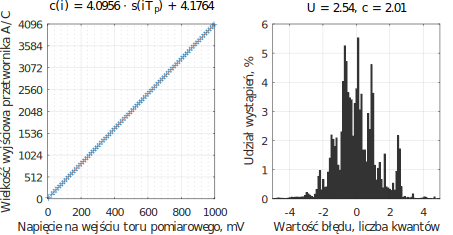
\includegraphics{obrazki/static_adcout}
\makecaption{fig:pom_static_fun}{Zależność wartości wielkości wyjściowej przetwornika analogowo-cyfrowego w funkcji wartości napięcia wejściowego analizowanego toru pomiarowego oraz histogram uzyskanych realizacji błędu losowego wielkości wyjściowej przetwornika analogowo-cyfrowego}
\end{center}
\end{figure}

Wykonany eksperyment pozwolił na identyfikację wypadkowego błędu przesunięcia zera wzmacniacza pomiarowego oraz przetwornika analogowo cyfrowego, który w analizowanym przypadku wyniósł \qty{0.123}{mV}. Błąd ten korygowany jest na etapie odtwarzania wartości wielkości $x(i)$ w przypadku warunków otoczenia identycznych do panujących podczas przeprowadzania eksperymentu. Na podstawie dokumentacji zastosowanych komponentów w rozważaniach należy uwzględnić zależność realizacji omawianego sygnału błędu w funkcji temperatury otoczenia. W przypadku wzmacniacza pomiarowego czułość błędu zera w funkcji temperatury otoczenia wynosi typowo \qty{\pm 2}{\micro V \per K} dla wzmocnienia statycznego na poziomie \qty{1}{V \per V}. W przypadku przetwornika analogowo-cyfrowego wartość ta nie jest przedstawiona w dokumentacji, natomiast producent układu proponuje wykonanie procedury kalibracji, a następnie na jej podstawie wykonywanie korekcji błędu przesunięcia zera stosując wbudowany przetwornik temperatury. Jako, że wszystkie eksperymenty związane z pracą przeprowadzane były przy stałej temperaturze otoczenia wynoszącej \qty{21}{\degreeCelsius}, analiza opisywanych zjawisk została pominięta. W przypadku zmiany wartości temperatury otoczenia należy przeprowadzić odpowiedni eksperyment mający na celu identyfikację czułości sygnału błędu związanego z dryfem zera w funkcji temperatury otoczenia, a następnie korygować należy wyniki pomiaru lub uwzględniać udział omawianego sygnału błędu w budżecie niepewności. 

Analizując dokumentacje~\cite{microchip_manual, stm_manual, diodes_manual, stm_f411} kolejnych komponentów toru pomiarowego zauważyć można, że najistotniejsze źródło błędów związanych z właściwościami statycznymi stanowi w analizowanym przypadku przetwornik analogowo-cyfrowy. Zgodnie z dokumentacją~\cite{stm_f411}, typowa wartość błędu granicznego wielkości wyjściowej $c(i)$ dla zbliżonych do stosowanych w sporządzonej aplikacji parametrów pracy przetwornika analogowo-cyfrowego powinna mieścić się w przedziale $\pm<2; 3>~\unit{LSB}$. Najważniejsze źródła błędu, które zdefiniowane są przez producenta zastosowanego przetwornika analogowo-cyfrowego obejmują: błąd przesunięcia charakterystyki względem zera, błąd wzmocnienia, całkowy błąd nieliniowości i różnicowy błąd nieliniowości~\cite{stm_adc, stm_f411}. Uzyskana na drodze eksperymentu wartość niepewności rozszerzonej jest mniejsza od wartości wynikającej z opisanego w dokumentacji błędu granicznego ze względu na fakt, że skorygowany został błąd zera oraz błąd wzmocnienia. Przeprowadzony eksperyment pozwolił zidentyfikować wypadkowe parametry sumy opisanych sygnałów błędów, przy czym należy zauważyć, że ze względu niewielką w stosunku do rozdzielczości przetwornika liczbę serii pomiarowych, nie udało się uzyskać większości realizacji różnicowego błędu nieliniowości. Na podstawie wyników eksperymentu oraz informacji zawartych w dokumentach~\cite{stm_f411, stm_adc} można jednak przyjąć, że wartość niepewności $U_{c,rw}$ została oszacowana prawidłowo. Ze względu na niewielką liczbę realizacji różnicowego błędu nieliniowości można zakładać, że rzeczywisty rozkład błędu $e_{c,rw}(i)$ będzie rozkładem normalnym, co wynika z centralnego twierdzenia granicznego~\cite{jcgm_guide}.

Drugą grupę właściwości stanowią właściwości dynamiczne. Podobnie, jak w przypadku właściwości statycznych, istnieje możliwość ich identyfikacji pomiarowej, uzyskując kolejne realizacje wielkości wyjściowej $c(i)$. Przypadek właściwości dynamicznych jest jednak złożony i wymaga stosowania bardziej skomplikowanej procedury pomiarów -- konieczna bowiem jest odpowiednia synchronizacja przebiegu napięcia wejściowego toru pomiarowego z przebiegiem sygnału wyjściowego przetwornika analogowo-cyfrowego, w celu oszacowania różnicy pomiędzy fazami analizowanych sygnałów. Opisywana procedura jest zatem kłopotliwa, a dodatkowo podczas jej realizacji wprowadzany byłby kolejny błąd, związany z opisywaną synchronizacją. Wobec powyższych okoliczności proponuje się w pierwszej kolejności identyfikację właściwości dynamicznych zastosowanego wzmacniacza pomiarowego, a następnie ustalenie właściwości dynamicznych przetwornika analogowo-cyfrowego na podstawie jego dokumentacji~\cite{stm_f411}, która szczegółowo opisuje model tego przetwornika.

W przypadku wzmacniacza pomiarowego proponowana procedura identyfikacji jego właściwości polega na podawaniu na wejście analizowanego wzmacniacza napięcia sinusoidalnie zmiennego o zadanej pulsacji i stałej amplitudzie. Dla zadanych parametrów sygnału wejściowego $s(t)$ zmierzyć należy amplitudę sygnału wyjściowego $y(t)$ wzmacniacza, potrzebną do wyznaczenia jego wzmocnienia $K_{y}(\omega)$, oraz przesunięcie fazowe $\varphi_{y}(\omega)$ pomiędzy sygnałem wejściowym i wyjściowym. Pomiędzy omawianymi wielkościami zachodzą następujące relacje:
\begin{gather}
K_{y} \emb{\omega} = \frac{E_{wy} \emb{\omega}}{E_{we} \emb{\omega}} \label{eq:pom_dyn_amp}, \\
\varphi_{y} \emb{\omega} = \varphi_{wy} \emb{\omega} - \varphi_{we} \emb{\omega} = -\omega \cdot \Delta t \emb{\omega} \label{eq:pom_dyn_phi},
\end{gather}
gdzie w funkcji pulsacji $E_{wy}(\omega)$ jest amplitudą sygnału wyjściowego, $E_{we}(\omega)$ amplitudą sygnału wejściowego, $\varphi_{wy}(\omega)$ przesunięciem fazowym sygnału wyjściowego, $\varphi_{we}(\omega)$ przesunięciem fazowym sygnału wejściowego wzmacniacza, natomiast $\Delta t(\omega)$ opóźnieniem sygnału wyjściowego względem sygnału wejściowego.

Omawiany eksperyment przeprowadzono wykorzystując jako źródło napięcia wejściowego analizowanego wzmacniacza generator przebiegów arbitralnych RIGOL DG1011~\cite{rigol_fawg}. W celu oszacowania wartości parametrów opisanych równaniami~\eqref{eq:pom_dyn_amp} oraz~\eqref{eq:pom_dyn_phi} zastosowano oscyloskop RIGOL DS5062MA~\cite{rigol_dso} w połączeniu z dwiema identycznymi sondami P6100~\cite{wellzion_probes}. Ze względu na zastosowanie dwóch identycznych sond pomiarowych obecne w zmierzonym wzmocnieniu i przesunięciu fazowym błędy były identyczne dla obydwóch kanałów, a zatem w równaniach~\eqref{eq:pom_dyn_amp} oraz~\eqref{eq:pom_dyn_phi} wzajemnie się kompensowały. Ze względu na pomiar amplitudy sygnału zarówno dla napięcia wejściowego, jak i wyjściowego analizowanego wzmacniacza, ewentualna rozbieżność nastawy wartości amplitudy napięcia wyjściowego generatora była nieistotna. Ze względu na bardzo małą wartość błędu nastawy częstotliwości przyjmuje się, że rzeczywista wartość częstotliwości sygnału wyjściowego generatora jest równa wartości zadanej tej częstotliwości. Podczas pomiarów analizowano uśrednione wartości dla $256$ realizacji obserwowanych sygnałów.

Na podstawie pozyskanych danych oszacowano pasmo przenoszenia analizowanego wzmacniacza, któremu dla zastosowanej konfiguracji układu odpowiadała częstotliwość graniczna $f_{y,g} \approx \qty{175}{kHz}$ oraz wzmocnienie statyczne $s_{y,a} \approx \qty{3.3}{V \per V}$. Dla przedstawionych charakterystyk sporządzono dwa modele, mające na celu przybliżenie właściwości analizowanego obiektu w zakresie częstotliwości $f \in~<0;\frac{1}{2}f_{p}>$. W modelu pierwszym wykorzystano funkcję opisującą transmitancję wzmacniacza w postaci:
\begin{gather}
\tilde{G}_{y,a} \emb{j\omega} = \frac{s_{y,a}}{1 + j \frac{\omega}{2 \pi f_{y,g}}} = \frac{s_{y,a}}{\frac{\omega^{2}}{4 \pi^{2} f_{y,g}^{2}} + 1} - j \frac{\omega s_{y,a}}{2 \pi f_{y,g} \left( \frac{\omega^{2}}{4 \pi^{2} f_{y,g}^{2}} + 1 \right) } \label{eq:pom_dyn_trans},
\end{gather}
natomiast dla modelu drugiego wykonano metodą najmniejszych kwadratów aproksymacje wielkości opisanych równaniami~\eqref{eq:pom_dyn_amp} oraz~\eqref{eq:pom_dyn_phi} przy użyciu funkcji:
\begin{gather}
\tilde{K}_{y,b} \emb{\omega} = 3.395 - 0.125 \exp \emb{\num{1.789e-6} \omega} \label{eq:pom_aprox_amp}, \\
\tilde{\varphi}_{y,b} \emb{\omega} = -\frac{1.700 \omega^{5}}{\num{e30}} + \frac{6.517 \omega^{4}}{\num{e24}} - \frac{7.932 \omega^{3}}{\num{e18}} + \frac{2.921 \omega^{2}}{\num{e12}} - \frac{6.924 \omega}{\num{e07}} \label{eq:pom_aprox_phi}.
\end{gather}
Uzyskane dla sygnału o częstotliwościach z zakresu $f \in~<0.1; 24>~\unit{kHz}$ wartości wzmocnienia i przesunięcia fazowego oraz odpowiadające im aproksymacje dla modeli opisanych w równaniach od~\eqref{eq:pom_dyn_trans} do~\eqref{eq:pom_aprox_phi} przedstawiono na rysunku~\ref{fig:pom_dynamic_ampout}.

\begin{figure}[htb!]
\begin{center}
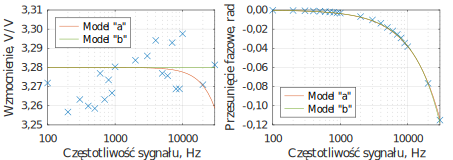
\includegraphics{obrazki/dynamic_ampout}
\makecaption{fig:pom_dynamic_ampout}{Zależność wartości wzmocnienia oraz przesunięcia fazowego w funkcji częstotliwości dla zastosowanej konfiguracji wzmacniacza pomiarowego}
\end{center}
\end{figure}

Analizując przedstawione wykresy zauważyć można, że model zaproponowany w równaniach~\eqref{eq:pom_aprox_amp} oraz~\eqref{eq:pom_aprox_phi} stanowi akceptowalne przybliżenie charakterystyki analizowanego wzmacniacza pomiarowego, natomiast model dany równaniem~\eqref{eq:pom_dyn_trans} odbiega od niej znacząco, przez co nie może być stosowany. Wobec powyższych przyjmuje się, że równania~\eqref{eq:pom_aprox_amp} oraz~\eqref{eq:pom_aprox_phi} opisywać będą właściwości dynamiczne zastosowanego wzmacniacza, odpowiadające zależnościom~\eqref{eq:mid_cont_amp} oraz~\eqref{eq:mid_cont_phi}, a zatem zachodzi $\tilde{K}_{y}(\omega) = \tilde{K}_{y,b}(\omega)$ oraz $\tilde{\varphi}_{y}(\omega) = \tilde{\varphi}_{y,b}(\omega)$. Należy zauważyć, że na potrzeby zaproponowanego w pracy modelu błędu pozyskane w wyniku przeprowadzonego eksperymentu informacje będą wystarczające i nie jest konieczna znajomość dokładnej postaci funkcji opisującej transmitancję analizowanego obiektu.

Ostatni etap identyfikacji właściwości dynamicznych obejmuje właściwości przetwornika analogowo-cyfrowego. Zgodnie z dokumentacją~\cite{stm_f411} obwód zastępczy części analogowej przetwornika analogowo-cyfrowego przedstawić można w postaci modelu filtra dolno-przepustowego typu \enquote{RC}, przy czym stanowić on będzie kaskadowe połączenie dwóch takich filtrów, co przedstawiono na rysunku~\ref{fig:pom_schemat_adc}. Wypadkowa pojemność $C_{we}$ wynika w analizowanym przypadku z pojemności w obrębie wyprowadzenia mikrokontrolera, natomiast pojemność $C_{adc}$ wynika pojemności wewnętrznej układu próbkująco-pamiętającego. Zgodnie z dokumentacją wewnętrzna pojemność przetwornika wynosi typowo około~\qty{4}{pF}, natomiast pojemność zastępcza $C_{we}$ obwodu wejściowego przetwornika wynosi zwykle około~\qty{5}{pF}. Rezystancję $R_{we}$ w zaproponowanym modelu stanowi szeregowe połączenie rezystancji doprowadzeń pomiędzy wzmacniaczem pomiarowym i mikrokontrolerem oraz rezystancji wyjściowej wzmacniacza, przy czym w omawianym przypadku jest to wartość rzędu pojedynczych Ohmów. Rezystancja $R_{adc}$ jest rezystancją klucza układu próbkująco-pamiętającego i, zgodnie z dokumentacją, jej wartość nie przekracza~\qty{6}{k\ohm}. Dodatkowe elementy, które można zauważyć na omawianym schemacie, to diody zabezpieczające wejście mikrokontrolera przed zbyt wysokim lub zbyt niskim napięciem wejściowym oraz źródło $I_{adc}$, które zastępuje upływność układu nieprzekraczającą~\qty{\pm 1}{\micro A}. Elementy te mogą być pominięte w omawianej analizie, ze względu na ich znikome znaczenie w budżecie błędów analizowanego toru pomiarowego.

\begin{figure}[htb!]
\begin{center}
\includegraphics{obrazki/schemat_adc}
\makecaption{fig:pom_schemat_adc}{Schemat zastępczy modelu przetwornika analogowo-cyfrowego zastosowanego w analizowanym torze pomiarowym zgodny z dokumentacją producenta układu~\cite{stm_f411}}
\end{center}
\end{figure}

Pierwszy filtr, który przedstawiono na rysunku~\ref{fig:pom_schemat_adc}, składa się z rezystancji rzędu pojedynczych Ohmów oraz pojemności rzędu mikro Faradów. Pozwala to oszacować częstotliwość graniczną tego filtru na poziomie kilkuset giga Herców. Filtr drugi stanowi połączenie rezystancji rzędu kilo Ohmów z pojemnością rzędu piko Faradów, a zatem rząd wielkości częstotliwości granicznej takiego filtru oszacować można na poziomie kilkuset mega Herców. Na podstawie przedstawionych parametrów modelu analizowanego przetwornika analogowo-cyfrowego, przyjąć można pomijalnie mały udział jego właściwości dynamicznych w puli właściwości dynamicznych całego toru pomiarowego. Ostateczna analiza właściwości dynamicznych całości toru pomiarowego uwzględniać może jedynie właściwości dynamiczne zastosowanego wzmacniacza pomiarowego, którego pasmo przenoszenia jest znacznie niższe.

Ostatnim fragmentem toru pomiarowego, który wprowadzać może do sygnału wyjściowego dodatkowe błędy, jest algorytm dyskretnej transformacji falkowej. Przeprowadzone wcześniej badania, których wyniki przedstawiono w tabeli~\ref{tab:varnum_spline4_4_5_f32}, pozwalają przypuszczać, że wariancja błędu związanego z zaokrągleniami nie przekroczy w bieżącym przypadku rzędu piko woltów, a zatem niepewność rozszerzona z nią związana nie powinna przekroczyć rzędu mikro woltów. Oznacza to, że błędy własne zastosowanego algorytmu dyskretnej transformacji falkowej mogą być pominięte w budżecie niepewności, bez większego wpływu na oszacowaną wartość niepewności rozszerzonej wielkości wyjściowych analizowanego toru pomiarowego~\cite{jcgm_guide}.

Należy zaznaczyć, że z punktu widzenia proponowanego modelu błędu dokładna znajomość postaci funkcji przetwarzania statycznego każdego elementu toru pomiarowego nie jest znana. Przykładowo, pomimo udziału funkcji przetwarzania $f_{y}(x)$ wzmacniacza pomiarowego w równaniach~\eqref{eq:pom_func_static} oraz~\eqref{eq:pom_funx_static}, znajomość tej funkcji nie jest konieczna podczas omawianej analizy. Dodatkowo, na podstawie treści przedstawionych równań zauważyć można, że na etapie przetwarzania wielkości $c(i)$ wprowadzane jest przesunięcie charakterystyki statycznej, spowodowane błędem zera wzmacniacza pomiarowego i przetwornika analogowo-cyfrowego. Opisywana sytuacja powoduje, że funkcja przetwarzania nie spełnia właściwości addytywności, przez co nie jest możliwa analiza każdego sygnału błędu z osobna, jak proponowano w opisanym w pracy modelu błędu. Przeprowadzenie analizy z punktu widzenia wielkości wejściowej algorytmu dyskretnej transformacji falkowej umożliwia eliminację opisywanych niedogodności i wykorzystanie równań od~\eqref{eq:out_disc_err_stat_self} do~\eqref{eq:out_disc_err_rand_prop}, umożliwiających analizę z zastosowaniem metody superpozycji dla obecnych w torze pomiarowym sygnałów.

\section{Model błędu toru pomiarowego}

Przyjmując założoną wcześniej czułość dla wielkości $x(i)$ w stosunku do przetwarzanego sygnału $s(t)$ równą $s_{s,x} = \qty{1}{V \per V}$, idealny oraz zakłócony sygnałem błędu przebieg wielkości $x(i)$ opisać można w postaci:
\begin{gather}
\dot{x} \emb{i} = s_{s,x} \dot{s} \emb{kT_{p}} = \dot{s} \emb{kT_{p}} \label{eq:pom_dwtina_ideal}, \\
\tilde{x} \emb{i} = \dot{s} \emb{kT_{p}} + e_{x,\Sigma} \emb{i} \label{eq:pom_dwtina_real}.
\end{gather}
Należy zauważyć, że sygnał błędu $e_{x,\Sigma}(t)$ zawierać będzie składowe związane z właściwościami statycznymi oraz dynamicznymi analizowanego toru pomiarowego, przy czym z osobna rozpatrywane będą sygnały związane z błędami własnymi, wprowadzanymi przez obiekt, oraz propagowanymi z wejścia na wyjście obiektu.

Uwzględniając założenie odnośnie czułości wielkości $x(i)$ względem sygnału $s(t)$ wynikające z wartości wzmocnienia statycznego $\tilde{K}_{y}(0)$ oraz postaci funkcji odtwarzania statycznego danych w równaniach~\eqref{eq:pom_funx_static} oraz~\eqref{eq:pom_aprox_amp} przyjmuje się, że wzmocnienie dla wielkości $x(t)$ względem wielkości $s(t)$ wprowadzane przez wzmacniacz pomiarowy wynosi w zakresie częstotliwości $f \in~<0; \frac{1}{2} f_{p}>$:
\begin{equation}
\tilde{K}_{s,x} \emb{\omega} = \frac{\tilde{K}_{y} \emb{\omega}}{\tilde{K}_{y} \emb{0}} \cong \qty{1}{V \per V} \label{eq:pom_dwtin_amp}.
\end{equation}
Na podstawie wypadkowych właściwości dynamicznych obiektu, wynikających z właściwości wzmacniacza oraz przetwornika analogowo-cyfrowego, można natomiast przyjąć, że przesunięcie fazowe sygnału $x(i)$ względem sygnału $s(t)$ jest dane zależnością:
\begin{equation}
\tilde{\varphi}_{s,x} \emb{\omega} = \tilde{\varphi}_{y} \emb{\omega} = -\frac{1.700 \omega^{5}}{\num{e30}} + \frac{6.517 \omega^{4}}{\num{e24}} - \frac{7.932 \omega^{3}}{\num{e18}} + \frac{2.921 \omega^{2}}{\num{e12}} - \frac{6.924 \omega}{\num{e07}} \label{eq:pom_dwtin_phi}.
\end{equation}

Pierwszy składnik zawarty w sygnale błędu $e_{x,\Sigma}(t)$ stanowi sygnał związany ze zidentyfikowanymi właściwościami statycznymi analizowanego wcześniej fragmentu toru pomiarowego, opisany dla warunków wykonanego eksperymentu równaniem~\eqref{eq:pom_funx_error}. Jako, że deterministyczna postać omawianego sygnału błędu nie jest znana oraz wartości jego realizacji nie zależą od częstotliwości przetwarzanego sygnału, przyjmuje się, że sygnał ten zalicza się do puli błędów losowych własnych. Niepewność rozszerzona związana z omawianym sygnałem błędu wynosi, zgodnie z poprzednimi rozważaniami, $U_{x,rw} = \qty{0.62}{mV}$ oraz przyjmuje się normalny rozkład realizacji tego błędu.

Drugi składnik sygnału błędu $e_{x,\Sigma}(t)$ stanowi sygnał związany z właściwościami dynamicznymi wzmacniacza pomiarowego, przy czym błąd ten ma charakter deterministyczny i można podzielić go na sygnał związany z błędem własnym oraz propagowanym. Analizując założenie opisane równaniem~\eqref{eq:pom_dwtin_amp} oraz charakterystykę amplitudową przedstawioną na rysunku~\ref{fig:pom_dynamic_ampout} zauważyć można, że dla zakresu częstotliwości $f \in~<0; \frac{1}{2} f_{p}>$ wartość wzmocnienia $\tilde{K}_{s,x}(\omega)$ jest stała, a zatem parametr ten nie ma wpływu na wprowadzane i przetwarzane sygnały błędów dynamicznych. Wobec powyższych, zgodnie z równaniami~\eqref{eq:mid_disc_err_dyn_self}, \eqref{eq:mid_disc_err_dyn_prop}, \eqref{eq:pom_funx_static} oraz~\eqref{eq:pom_dwtin_amp}:
\begin{gather}
\begin{split}
e_{x,dw} \emb{i} =~
& \sum _{j = 1} ^{\infty} E_{s,o} \emb{\omega_{x,j}} \sin \left( \omega_{s,j} iT_{p} + \varphi_{s,o} \emb{\omega_{s,j}} + \tilde{\varphi}_{s,x} \emb{\omega_{s,j}} \right) - \\
& \sum _{k = 1} ^{\infty} E_{s,o} \emb{\omega_{x,k}} \sin \left( \omega_{s,k} iT_{p} + \varphi_{s,o} \emb{\omega_{s,k}} + \dot{\varphi}_{s,x} \emb{\omega_{s,k}} \right)
\end{split}
\label{eq:pom_errx_dyn_self}, \\
e_{x,dp} \emb{i} = \sum _{j = 1} ^{\infty} E_{s,e} \emb{\omega_{s,j}} \sin \left( \omega_{s,j} iT_{p} + \varphi_{s,e} \emb{\omega_{s,j}} + \tilde{\varphi}_{s,x} \emb{\omega_{s,j}} \right) \label{eq:pom_errx_dyn_prop},
\end{gather}
przy czym stosowane oznaczenia parametrów sygnału $s(t)$ są zbieżne z tymi wprowadzonymi w równaniach od~\eqref{eq:in_cont_sum_ideal} do~\eqref{eq:in_cont_err_dyn} oraz $\dot{\varphi}_{s,x}(\omega) = \qty{0}{rad}$.

Trzeci składnik sygnału błędu $e_{x,\Sigma}(t)$ wynika z wpływu analizowanego obiektu na obecny w przetwarzanym sygnale $s(t)$ sygnał błędu statycznego $e_{s,s}(t)$, przy czym przebieg tego sygnału na wyjściu obiektu opisać można zgodnie z równaniem~\eqref{eq:pom_funx_static} jako:
\begin{equation}
e_{x,sp} \emb{i} = e_{s,s} \emb{i T_{p}} \label{eq:pom_errx_stat_prop}.
\end{equation}
Oznacza to, że zgodnie z równaniami~\eqref{eq:mid_disc_var_omega} oraz~\eqref{eq:out_disc_var_sense}, wariancję tego sygnału opisać można następującą zależnością:
\begin{equation}
\sigma_{x,sp}^{2} = s_{s,x}^{2} \tilde{K}_{s,x}^{2} \emb{0} \sigma_{s,s}^{2} \cong \sigma_{s,s}^{2} \label{eq:pom_varx_stat_prop}.
\end{equation}
Jako, że przeprowadzone eksperymenty wykonano przy stałych parametrach otoczenia, nie obejmowały one identyfikacji źródeł i postaci sygnału błędu statycznego własnego. Przyjmuje się zatem, że $e_{x,sw}(i) = 0$ oraz $\sigma_{x,sw}^{2} = 0$.

Czwartym składnikiem sygnału błędu $e_{x,\Sigma}(t)$ jest propagowany sygnał błędu losowego $e_{s,r}(t)$. Zgodnie z zależnościami~\eqref{eq:mid_disc_var_omega} oraz~\eqref{eq:out_disc_var_sense} dla założenia danego równaniem~\eqref{eq:pom_dwtin_amp} wariancję tego sygnału opisać można w postaci:
\begin{equation}
\sigma_{x,rp}^{2} = s_{s,x}^{2} \tilde{K}_{s,x}^{2} \emb{\omega} \sigma_{s,r}^{2} \emb{\omega} \cong \sigma_{s,r}^{2} \emb{\omega} \label{eq:pom_varx_rand_prop},
\end{equation}
co przy założeniu~\eqref{eq:pom_dwtina_ideal} odnośnie liniowości tego obiektu oznacza, że obiekt ten nie ma wpływu na widmo sygnałów losowych w zakresie częstotliwości $f \in~<0; \frac{1}{2} f_{p}>$, zatem:
\begin{equation}
e_{x,rp} \emb{i} \cong e_{x,r} \emb{i} \cong e_{s,r} \emb{i T_{p}} \label{eq:pom_errx_rand_prop}.
\end{equation}
W przypadku sygnału losowego błędu własnego $e_{x,rw}(i)$ przeprowadzony eksperyment pozwolił oszacować wariancję tego sygnału $\sigma_{x,rw}^{2} = \qty{0.095}{\micro V}$ oraz związaną z nią niepewność $U_{x,rw} = \qty{0.62}{mV}$, gdzie zakłada się $c_{x,rw} = c_{n} = 1.96$.

Na podstawie zależności od~\eqref{eq:pom_dwtina_ideal} do~\eqref{eq:pom_errx_rand_prop} wypadkowy sygnał błędu $e_{x,\Sigma}(t)$ opisać można jako sumę zdefiniowanych dotychczas sygnałów błędów cząstkowych w postaci:
\begin{equation}
e_{x,\Sigma} \emb{i} = e_{x,sp} \emb{i} + e_{x,dw} \emb{i} + e_{x,dp} \emb{i} + e_{x,rw} \emb{i} + e_{x,rp} \emb{i} \label{eq:pom_errx_sum},
\end{equation}
przy czym wypadkowe sygnały błędów z uwzględnieniem podziału na zaproponowane kategorie można zdefiniować jako:
\begin{gather}
e_{x,s} \emb{i} = e_{x,sp} \emb{i} \label{eq:pom_errx_stat}, \\
e_{x,d} \emb{i} = e_{x,dw} \emb{i} + e_{x,dp} \emb{i} = \sum _{j=1} ^{\infty} E_{x,e} \emb{\omega_{x,j}} \sin \emb{i T_{p} \omega_{x,j} + \varphi_{x,e} \emb{\omega_{x,j}}} \label{eq:pom_errx_dyn}, \\
e_{x,r} \emb{i} = e_{x,rw} \emb{i} + e_{x,rp} \emb{i} \label{eq:pom_errx_rand},
\end{gather}
gdzie wypadkowe parametry amplitudy $E_{x,e}(\omega_{x,j})$ oraz fazy $\varphi_{x,e}(\omega_{x,j})$ dla kolejnych harmonicznych sygnału wypadkowego błędu dynamicznego $e_{x,d}(i)$ zależne będą od widma przetwarzanego sygnału, natomiast ich wyznaczenie przebiegać będzie zgodnie z metodologią opisaną w równaniach od~\eqref{eq:dyn_vect} do~\eqref{eq:dyn_vect_phi}. Wariancję kolejnych harmonicznych sygnału $e_{x,d}(i)$ wyznaczyć można zgodnie z zależnością~\eqref{eq:dyn_var}.

Przedstawiona aplikacja zaproponowanego w pracy modelu błędu wielkości wejściowych algorytmu dyskretnej transformacji falkowej umożliwia określenie wariancji każdego z wymienionych w równaniu~\eqref{eq:pom_errx_sum} sygnałów oraz wyznaczenie niepewności rozszerzonej związanej z tymi sygnałami. W przypadku sygnałów błędów statycznych i losowych dla $i-tej$ wielkości wyjściowej toru pomiarowego zachodzi:
\begin{gather}
\sigma_{i,s}^{2} = \left| H_{i} \emb{0} \right|^{2} = A_{i,s}^{2} \sigma_{x,s}^{2} \label{eq:pom_varout_stat}, \\
\sigma_{i,r}^{2} = A_{i,r}^{2} \sigma_{x,r}^{2} \label{eq:pom_varout_rand}, 
\end{gather}
co wynika bezpośrednio z zależności opisanych równaniami od~\eqref{eq:alg_outvar_stat} do~\eqref{eq:alg_outvar_trans_rand} oraz założenia dotyczącego stałej widmowej gęstości mocy w przypadku sygnałów błędu kwantowania i wypadkowego błędu niedoskonałości charakterystyki statycznej. W przypadku sygnałów błędów dynamicznych, wariancję tych sygnałów w funkcji pulsacji opisać można równaniem:
\begin{equation}
\sigma_{i,d}^{2} \emb{\omega} = \left| H_{i} \emb{\omega T_{p}} \right|^{2} \sigma_{x,d}^{2} \emb{\omega} \label{eq:pom_varout_dyn},
\end{equation}
natomiast wypadkowa wariancja sygnału błędu dynamicznego może zostać opisana w postaci sumy wypadkowych wariancji wszystkich harmonicznych tego sygnału:
\begin{equation}
\sigma_{i,d}^{2} = \sum _{j=1} ^{\infty} \left| H_{i} \emb{\omega_{x,j} T_{p}} \right|^{2} \sigma_{x,d}^{2} \emb{\omega_{x,j}} \label{eq:pom_varout_dyn_sum}.
\end{equation}
Należy zauważyć, że na etapie analizy kolejnych harmonicznych sygnału błędu dynamicznego $e_{x,d}(i)$ kolejne harmoniczne tego sygnału mogą być ze sobą skorelowane. Proponowane w równaniu~\eqref{eq:pom_errx_dyn} przedstawienie tego sygnału w postaci kolejnych harmonicznych o parametrach wypadkowych umożliwia rozpatrzenie tych korelacji przy jednoczesnej redukcji liczby składowych analizowanego sygnału. Ze względu na to, że przeprowadzona identyfikacja właściwości metrologicznych dla fragmentu toru pomiarowego związanego z wielkościami wejściowymi analizowanego algorytmu nie wykazała innych korelacji pomiędzy zidentyfikowanymi sygnałami błędów, zgodnie z równaniem~\eqref{eq:var_matrix} zapisać można:
\begin{equation}
\sigma_{i,\Sigma}^{2} = \sigma_{i,s}^{2} + \sigma_{i,d}^{2} + \sigma_{i,r}^{2} \label{eq:pom_varout_sum}.
\end{equation}
Wartości wariancji sygnałów propagowanego błędu statycznego, propagowanego błędu losowego oraz wypadkowego błędu dynamicznego nie są znane na obecnym etapie analizy. Dla wymienionych sygnałów wartość wariancji zależeć będzie od widma sygnału $s(t)$ oraz zawartych w nim sygnałów błędów.

Wartości niepewności rozszerzonych związane z wymienionymi sygnałami błędów na wyjściu algorytmu mogą być w analizowanej sytuacji opisane jako:
\begin{gather}
U_{i,s} = c_{x,s} \sigma_{i,s} \label{eq:pom_uncout_stat}, \\
U_{i,d,j} = c_{d} \sigma_{i,d} \emb{\omega_{x,j}} \label{eq:pom_uncout_dyn}, \\
U_{i,r} = c_{n} \sigma_{i,r} \label{eq:pom_uncout_rand},
\end{gather}
gdzie zgodnie ze zidentyfikowanymi właściwościami obiektu $c_{x,s} = c_{n} = 1.96$. Wartość współczynnika rozszerzenia w przypadku sygnału błędu losowego na wyjściu obiektu wynika z założeń centralnego twierdzenia granicznego, gdzie analizowany algorytm przetwarza wiele nieskorelowanych ze sobą sygnałów błędów losowych o jednakowych parametrach. Wobec powyższych, wypadkowa wartość niepewności rozszerzonej na wyjściu algorytmu dla $i$-tej wielkości wyjściowej może być opisana zgodnie z równaniem~\eqref{eq:unc_matrix}, przy czym w analizowanym przypadku wektor niepewności sygnałów składowych opisać można jako:
\begin{equation}
\mathbf{U}_{i}^{T} = 
\begin{bmatrix}
U_{i,s} & U_{i,r} & U_{i,d,1} & U_{i,d,2} & \hdots & U_{i,d,K}
\end{bmatrix}
\label{eq:pom_uncout_uncvect},
\end{equation}
natomiast macierz koherencji dla $K$ harmonicznych sygnału błędu dynamicznego opisać można w postaci:
\begin{equation}
\mathbf{h}_{i} =
\begin{bmatrix}
1           & h_{i,s,r}   & h_{i,s,d,1} & h_{i,s,d,2} & \cdots & h_{i,s,d,K} \\
h_{i,r,s}   & 1           & h_{i,r,d,1} & h_{i,r,d,2} & \cdots & h_{i,r,d,K} \\
h_{i,d,1,s} & h_{i,d,1,r} & 1           & h_{i,d,1,2} & \cdots & h_{i,d,1,K} \\
h_{i,d,2,s} & h_{i,d,2,r} & h_{i,d,2,1} & 1           & \cdots & h_{i,d,2,K} \\
\vdots      &             &             &             & \ddots & \vdots      \\
h_{i,d,K,1} & \cdots      & \cdots      & \cdots      & \cdots & 1           \\
\end{bmatrix}
\label{eq:pom_uncout_cohers},
\end{equation}
gdzie kolejne wartości współczynników koherencji są wyznaczane zgodnie z równaniem~\eqref{eq:unc_coher}. Wobec przedstawionych założeń, wartość wypadkowej niepewności rozszerzonej dla analizowanego przypadku wynosi:
\begin{equation}
U_{i,\Sigma} = \sqrt{\mathbf{U}_{i}^{T} \mathbf{h}_{i} \mathbf{U}_{i}} \label{eq:pom_uncout_sum}.
\end{equation}
Zgodnie z założeniami odnośnie bardzo niskiej w stosunku do pozostałych sygnałów wariancji błędu własnego zaokrągleń, udział tego błędu pominięto w rozważaniach.

\section{Przypadek sygnału monoharmonicznego}

Pierwszym rozważanym eksperymentem jest weryfikacja poprawności przedstawionej aplikacji modelu błędu dla przypadku, kiedy analizowany tor pomiarowy przetwarza opisany równaniem~\eqref{eq:pom_gen_out_ideal} sinusoidalnie zmienny sygnał napięciowy. Eksperyment obejmuje dwa przypadki -- dla przypadku pierwszego nieznane są rzeczywiste wartości napięcia amplitudy $\tilde{E}_{s,o}$ oraz składowej stałej $\tilde{D}_{s,o}$ przetwarzanego sygnału $s(t)$, natomiast przypadek drugi zakłada znajomość tych parametrów, pozyskaną przy użyciu dodatkowego multimetru. Należy zaznaczyć, że w przypadku znajomości rzeczywistych parametrów przetwarzanego sygnału, wyznaczone analitycznie wartości wariancji oraz wypadkowej niepewności rozszerzonej dla kolejnych wielkości wyjściowych toru pomiarowego powinny być zbieżne z uzyskanymi na drodze eksperymentu. W przypadku analizy obejmującej nieznane rzeczywiste wartości parametrów sygnału $s(t)$ uzyskane analityczne wyniki powinny dotyczyć $95\%$ egzemplarzy stosowanego generatora przebiegów arbitralnych, a zatem ich wartości powinny być co najmniej takie, jakie uzyskano w eksperymencie.

W dalszej części przyjmuje się, że opisany równaniem~\eqref{eq:pom_gen_out_ideal} przebieg $s(t)$ w przypadku idealnym cechuje amplituda $\dot{E}_{s,o} = \qty{475}{mV}$ oraz składowa stała $\dot{D}_{s,o} = \qty{500}{mV}$, natomiast wartość pulsacji $\omega_{s,o}$ zależna jest od iteracji przeprowadzonego eksperymentu. Można zatem, na podstawie równań~\eqref{eq:pom_gen_shferr_unc} oraz~\eqref{eq:pom_gen_err_dyn_mono} wskazać graniczną wartość amplitudy sygnału błędu dynamicznego $e_{s,d}(t)$ dla analizowanych warunków eksperymentu:
\begin{equation}
E_{s,e,1} = U_{E} \emb{\dot{E}_{s,o}} = \frac{1.65}{\sqrt{3}} \emb{\num{5e-3} \cdot 0.475 + \num{0.5e-3}} = \qty{2.74}{mV} \label{eq:pom_mono_dyn_amp_in}.
\end{equation}
Na podstawie treści równania~\eqref{eq:pom_errx_dyn_prop} określić można amplitudę oraz fazę analizowanego sygnału błędu na wejściu algorytmu dyskretnej transformacji falkowej:
\begin{gather}
E_{x,ep,1} \cong E_{s,e,1} \label{eq:pom_mono_dyn_prop_amp_mid}, \\
\varphi_{x,ep,1,a} = \tilde{\varphi}_{s,x} \emb{\omega_{s,o}} + \left. \varphi_{s,e,1} \right|_{\tilde{E}_{s,o} - \dot{E}_{s,o} > 0} = \tilde{\varphi}_{s,x} \emb{\omega_{s,o}} \label{eq:pom_mono_dyn_prop_phi_mid_a}, \\
\varphi_{x,ep,1,b} = \tilde{\varphi}_{s,x} \emb{\omega_{s,o}} + \left. \varphi_{s,e,1} \right|_{\tilde{E}_{s,o} - \dot{E}_{s,o} < 0} = \tilde{\varphi}_{s,x} \emb{\omega_{s,o}} + \pi \label{eq:pom_mono_dyn_prop_phi_mid_b},
\end{gather}
przy czym faza $\varphi_{x,ep,1,a}$ jest odpowiednia dla dodatnich realizacji błędu nastawy amplitudy sygnału, natomiast faza $\varphi_{x,ep,1,b}$ odpowiada ujemnym realizacjom tego błędu. W przypadku sygnału błędu statycznego, wynikającego z błędu nastawy wartości składowej stałej $\dot{D}_{x,o}$ niepewność związaną z tym sygnałem określa zależność:
\begin{equation}
U_{x,sp} = c_{x,sp} \sigma_{x,sp} \cong c_{s,s} \sigma_{s,s} = U_{s,s} = \frac{1.65}{\sqrt{3}} \emb{\num{5e-3} \cdot 0.5 + \num{2e-3}} = \qty{4.29}{mV} \label{eq:pom_mono_stat_unc_mid},
\end{equation}
wynikająca z treści równań od~\eqref{eq:pom_gen_err_stat} do~\eqref{eq:pom_gen_unc_stat}, \eqref{eq:pom_errx_stat_prop} oraz \eqref{eq:pom_varx_stat_prop}. Wariancja omawianego sygnału błędu, zgodnie z wymienionymi zależnościami, wynosi natomiast:
\begin{equation}
\sigma_{x,sp}^{2} \cong \sigma_{s,s}^{2} = \sigma_{D}^{2} \emb{\dot{D}_{s,o}} = \frac{1}{3} \emb{\num{5e-3} \cdot 0.5 + \num{2e-3}}^{2} = \qty{6.75}{\micro V} \label{eq:pom_mono_stat_var_mid}.
\end{equation}
Równania od~\eqref{eq:pom_mono_dyn_amp_in} do~\eqref{eq:pom_mono_stat_unc_mid} dotyczą przypadku, gdy rzeczywiste wartości parametrów $\tilde{E}_{s,o}$ oraz $\tilde{D}_{s,o}$ nie są znane. Dla znanych wartości tych parametrów przyjmuje się, że $E_{s,e,1} = \qty{0}{V}$ oraz $U_{s,s} = \qty{0}{V}$, a zatem zachodzi $\sigma_{x,sp}^{2} = \qty{0}{V}$ oraz $\sigma_{x,dp}^{2} = \qty{0}{V}$.

Na podstawie równania~\eqref{eq:pom_errx_dyn_self} wyróżnić można dwie składowe harmonicznej sygnału błędu dynamicznego własnego na wejściu algorytmu transformacji falkowej. Amplitudy oraz fazy tych harmonicznych w analizowanym przypadku opisać można jako:
\begin{gather}
E_{x,ew,1,1} = E_{x,ew,1,2} \cong \dot{E}_{s,o} \label{eq:pom_mono_dyn_self_amp_mid}, \\
\varphi_{x,ew,1,1} = \varphi_{s,o} + \tilde{\varphi}_{s,x} \emb{\omega_{s,o}} = \tilde{\varphi}_{s,x} \emb{\omega_{s,o}} \label{eq:pom_mono_dyn_self_phi_mid_1}, \\
\varphi_{x,ew,1,2} = \varphi_{s,o} + \dot{\varphi}_{s,x} \emb{\omega_{s,o}} + \pi = \pi \label{eq:pom_mono_dyn_self_phi_mid_2},
\end{gather}
gdzie na podstawie założeń danych równaniem~\eqref{eq:pom_gen_out_ideal} $\varphi_{s,o} = \qty{0}{rad}$ oraz zgodnie z założeniem~\eqref{eq:pom_dwtina_ideal} $\dot{\varphi}_{s,x}(\omega) = \qty{0}{rad}$. Zgodnie z definicją sygnału błędu dynamicznego $e_{x,d}(i)$ daną równaniem~\eqref{eq:pom_errx_dyn}, wynikającą z definicji~\eqref{eq:pom_errx_dyn_self} oraz~\eqref{eq:pom_errx_dyn_prop}, w analizowanym przypadku zapisać można:
\begin{equation}
\begin{split}
e_{x,d,*} \emb{i} =~
& E_{x,ew,1,2} \sin \emb{\omega_{s,o} + \varphi_{x,ew,1,2}} + E_{x,ew,1,1} \sin \emb{\omega_{s,o} + \varphi_{x,ew,1,1}} + \\
& E_{x,ep,1} \sin \emb{\omega_{s,o} + \varphi_{x,ep,1,*}} = E_{x,e,1,*} \sin \emb{\omega_{s,o} + \varphi_{x,e,1,*}}
\end{split}
\label{eq:pom_mono_dyn_sum_err_mid},
\end{equation}
gdzie rozpatrzyć należy obydwa przypadki amplitudy $E_{x,e,1,*}$ oraz fazy $\varphi_{x,e,1,*}$ sygnału propagowanego błędu dynamicznego $e_{x,dp}(i)$ dla wariantów parametru $\varphi_{x,ep,1,*}$, którego wartości w zależności od zaistniałych okoliczności opisano w równaniach~\eqref{eq:pom_mono_dyn_prop_phi_mid_a} oraz~\eqref{eq:pom_mono_dyn_prop_phi_mid_b}. Zgodnie z metodologią opisaną w równaniach~od~\eqref{eq:dyn_vect} do~\eqref{eq:dyn_vect_phi} wartości parametrów amplitudy $E_{x,e,1}$ oraz fazy $\varphi_{x,e,1}$ sygnału błędu dynamicznego $e_{x,d}(i)$ na wejściu algorytmu dyskretnej transformacji falkowej mogą być wyznaczone jako:
\begin{gather}
E_{x,e,1,*} = \sqrt{e_{x,1,\Sigma,a,*}^{2} + e_{x,1,\Sigma,b,*}^{2}} \label{eq:pom_mono_dyn_sum_param_amp_mid}, \\
\varphi_{x,e,1,*} = \arctan \emb{\frac{e_{x,1,\Sigma,a,*}^{2}}{e_{x,1,\Sigma,b,*}^{2}}} \label{eq:pom_mono_dyn_sum_param_phi_mid},
\end{gather}
przy czym parametry przedstawionych równań wyznaczane są zgodnie z zależnościami:
\begin{gather}
\begin{split}
e_{x,1,\Sigma,a,*} =~ & E_{x,ew,1,2} \cos \emb{\varphi_{x,ew,1,2}} + E_{x,ew,1,1} \cos \emb{\varphi_{x,ew,1,1}} + \\ & E_{x,ep,1} \cos \emb{\varphi_{x,ep,1,*}}
\end{split}
\label{eq:pom_mono_dyn_sum_param_a_mid}, \\
\begin{split}
e_{x,1,\Sigma,b,*} =~ & E_{x,ew,1,2} \sin \emb{\varphi_{x,ew,1,2}} + E_{x,ew,1,1} \sin \emb{\varphi_{x,ew,1,1}} + \\ & E_{x,ep,1} \sin \emb{\varphi_{x,ep,1,*}}
\end{split}
\label{eq:pom_mono_dyn_sum_param_b_mid}.
\end{gather}

Należy podkreślić, że rzeczywisty przebieg sygnału błędu dynamicznego własnego $e_{x,dw}(i)$ również skorelowany jest z rzeczywistą wartością amplitudy $\tilde{E}_{s,o}$. Korelacja ta jest jednak pominięta w przeprowadzonej analizie ze względu na niewielkie wartości błędu nastawy tego parametru i w efekcie niski współczynnik korelacji opisywanego zjawiska. Jest to założenie analogiczne, jak stosowanie idealnej charakterystyki przetwarzania obiektu w przypadku analizy statycznych właściwości tego obiektu.



\section{Podsumowanie przeprowadzonego eksperymentu}

TODO

